% Compile from the project root with tectonic COURSE_PROJECT_SLIDES_V2.tex.
% Rebuild figures with python scripts/build_slide_assets.py.
% The 19 numbered frames have a target running time of 18 minutes.
% Speaker notes are embedded with \note{} and hidden in the audience PDF.
\documentclass[aspectratio=169,11pt]{beamer}
\usepackage[T1]{fontenc}
\usepackage{lmodern,amsmath,amssymb,booktabs}
\usepackage{tikz}
\usetikzlibrary{positioning,arrows.meta,calc}
\usefonttheme{professionalfonts}
\definecolor{navy}{HTML}{16364A}
\definecolor{teal}{HTML}{007F83}
\definecolor{orange}{HTML}{C45A13}
\definecolor{muted}{HTML}{576574}
\setbeamercolor{normal text}{fg=navy,bg=white}
\setbeamercolor{structure}{fg=teal}
\setbeamercolor{frametitle}{fg=navy}
\setbeamercolor{block title}{fg=white,bg=navy}
\setbeamercolor{block body}{fg=navy,bg=navy!5}
\setbeamerfont{frametitle}{size=\Large,series=\bfseries}
\setbeamerfont{title}{size=\LARGE,series=\bfseries}
\setbeamertemplate{navigation symbols}{}
\setbeamertemplate{itemize items}[circle]
\setbeamersize{text margin left=8mm,text margin right=8mm}
\setbeamertemplate{footline}{%
  \hspace{8mm}\textcolor{muted}{\scriptsize\insertsectionhead}
  \hfill\textcolor{muted}{\scriptsize\insertframenumber/\inserttotalframenumber}
  \hspace{8mm}\vspace{3mm}}
\setbeamertemplate{frametitle}{\vspace{3mm}\insertframetitle\par\vspace{2mm}}
\setbeameroption{hide notes}
\newcommand{\norm}[1]{\lVert #1\rVert_2}
\newcommand{\tf}{f_\phi}
\newcommand{\source}[1]{\par\vfill{\color{muted}\tiny #1}}
\title{Stability and Information Sensitivity\\in Transformer In-Context Inverse Learning}
\author{Fei Zhang}
\institute{University of Waterloo\\CS 886}
\date{November 2026}


\begin{document}
\section{Motivation}

% 1. 0:00--0:25
\begin{frame}[plain]
\vfill
{\usebeamerfont{title}\inserttitle\par}
\vspace{6mm}
{\large Fei Zhang\par}
\vspace{2mm}
{\color{muted}University of Waterloo\quad CS 886\par}
\vspace{7mm}
{\color{teal}\large Can a stable Transformer use the one record that identifies a task?}
\vfill
\note{Target time 25 seconds, cumulative 0:25.
The question for this talk is what happens when almost all the useful
information about one parameter sits in a single observation. We examine
a frozen Transformer, first through a simple example and two complementary
bounds, then through controlled inverse-learning experiments.}
\end{frame}

% 2. 0:25--1:05
\begin{frame}{When should one observation change the answer?}
\begin{columns}[T,onlytextwidth]
\column{.47\textwidth}
{\large Ordinary replacement}
\vspace{3mm}

A different record from the same task.

\[
\theta'=\theta
\]

A small prediction change can accompany accurate recovery.
\column{.47\textwidth}
{\large Identifying replacement}
\vspace{3mm}

A record that distinguishes two tasks.

\[
\theta'\ne\theta
\]

Accurate recovery requires the prediction to change.
\end{columns}
\vspace{6mm}
\begin{block}{Research question}
Can a Transformer remain stable while responding enough to the observations
that determine the correct task parameters?
\end{block}
\note{Target time 40 seconds, cumulative 1:05.
Small sensitivity can mean different things. If I replace an observation
with another from the same task, the correct parameters stay the same,
so an unchanged prediction can be exactly right. If a replacement
distinguishes two different tasks, the correct answer changes.
An estimator that stays almost unchanged may then be wrong.
Our question is whether the model makes that distinction.
To make the distinction concrete, consider a line with an unknown slope.}
\end{frame}

% 3. 1:05--2:10
\begin{frame}{A single record can determine the slope}
\begin{columns}[c,onlytextwidth]
\column{.52\textwidth}
\[
y=bx
\]
{\small\setlength{\tabcolsep}{4pt}
\begin{tabular}{lcc}
\toprule
& Context A & Context B\\
\midrule
Shared \(m-1\) records & \((0,0)\) & \((0,0)\)\\
Last record & \((1,1)\) & \((1,2)\)\\
\midrule
Correct slope & \(b=1\) & \(b=2\)\\
\bottomrule
\end{tabular}
}
\vspace{4mm}

Each context identifies its slope.

Adding copies of \((0,0)\) supplies no new slope information.
\column{.44\textwidth}
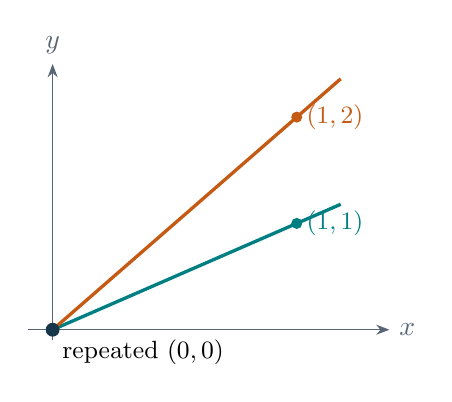
\begin{tikzpicture}[x=3.1cm,y=1.35cm,>=Stealth]
\draw[->,muted] (-.1,0)--(1.38,0) node[right]{\(x\)};
\draw[->,muted] (0,-.1)--(0,2.5) node[above]{\(y\)};
\draw[teal,very thick] (0,0)--(1.18,1.18);
\draw[orange,very thick] (0,0)--(1.18,2.36);
\fill[teal] (1,1) circle (2pt);
\fill[orange] (1,2) circle (2pt);
\fill[navy] (0,0) circle (2.5pt);
\node[teal,right,font=\small] at (1,1){\((1,1)\)};
\node[orange,right,font=\small] at (1,2){\((1,2)\)};
\node[below right,font=\small] at (0,0){repeated \((0,0)\)};
\end{tikzpicture}
\end{columns}
\vspace{4mm}
{\color{teal}\large Only one record changes, but the correct answer changes by 1.}
\note{Target time 65 seconds, cumulative 2:10.
Both contexts contain the same repeated zeros. Every line through
the origin is consistent with those zeros, so they tell us nothing
about the slope. The last record supplies the slope: one in A and
two in B. Each complete context has a unique correct answer.
Now imagine adding a thousand more copies of the zero record.
The answer still depends on that last observation just as strongly.
This is the example to keep in mind throughout the theory.
We will compare how much an architecture can respond with how much
accurate recovery requires it to respond.}
\end{frame}

% 4. 2:10--2:50
\begin{frame}{Possible response and required response}
Let \(\Delta=\norm{f(S)-f(S')}\) and \(D=\norm{\theta-\theta'}\).
\vspace{4mm}
\begin{columns}[T,onlytextwidth]
\column{.47\textwidth}
{\large Theorem 1: architecture}
\[
\Delta\le C/m
\]
How much can a fixed encoder change when one record changes?
\column{.47\textwidth}
{\large Theorem 2: recovery}
\[
\Delta\ge D-2\epsilon
\]
How much must any estimator change if both errors are at most \(\epsilon\)?
\end{columns}
\vspace{7mm}
{\color{teal}\large The two bounds concern the same response \(\Delta\).}
\source{The first bound adapts established Transformer stability reasoning.
The second follows from the triangle inequality.}
\note{Target time 40 seconds, cumulative 2:50.
There are two separate questions. Theorem one gives a ceiling on
the response permitted by the architecture. Theorem two gives a
floor on the response required for accuracy. Delta is the same
prediction difference in both statements. D is the distance between
the correct parameters. Neither statement says that a smaller
response is always better. Before proving them, I will define the
inverse-learning model to which we apply these questions.}
\end{frame}

\section{Methodology}
% 5. 2:50--4:05
\begin{frame}{Learning cost parameters from dispatch observations}
\begin{columns}[T,onlytextwidth]
\column{.49\textwidth}
{\large The task}
\[
\min_{\substack{x_1+x_2=d\\0\le x_i\le1}}
\sum_{i=1}^2\left(a_ix_i+\tfrac12b_ix_i^2\right).
\]
Unknown costs:
\[
\theta=(a_1,b_1,a_2,b_2).
\]
Observed record:
\[
z_t=(d_t,x_{1t},x_{2t},\lambda_t,s_{1t},s_{2t}).
\]
\column{.47\textwidth}
{\large Interior KKT information}\par\vspace{1mm}
For an interior generator, KKT gives
\[
\lambda_t=a_i+b_ix_{it}.
\]
This is affine regression.

\vspace{3mm}
Two distinct interior outputs identify the two coefficients.

\vspace{3mm}
A bound status supplies an inequality.
\end{columns}
\vspace{1mm}
\[
S_m
\ \xrightarrow{\ \text{2-layer Transformer}\ }\ H
\ \xrightarrow{\ \text{mean pooling and head}\ }\ \widehat\theta.
\]
\source{Supervised source-task training. Weights stay fixed on unseen tasks.
Two unit-capacity generators, positive bounded cost slopes.}
\note{Target time 75 seconds, cumulative 4:05.
Each synthetic task has four unknown cost coefficients. For a given
demand we observe optimal generator outputs, a clearing price, and
whether each output is at a bound. The price equals marginal cost
for an interior generator. This produces exactly the affine equation
from the motivating example. Two different interior outputs identify
that generator's intercept and slope. Bound observations instead
give one-sided inequalities. A two-layer Transformer reads complete
market records, averages its final token states, and predicts four
cost coefficients through a bounded head. We train it on labeled
source tasks, then freeze it on new tasks. The question is how its
context response relates to the information in these equations.
We first establish an architectural upper bound.}
\end{frame}

% 6. 4:05--4:55
\begin{frame}{Theorem 1: a fixed encoder has a \(C/m\) response bound}
\begin{block}{Encoder replacement stability}
Fix finite weights and depth, bounded records, full attention,
a mean-pooled Lipschitz readout, and positive LayerNorm epsilon.
Then a finite \(C\), independent of \(m\), satisfies
\[
\boxed{\norm{f_\phi(S_m)-f_\phi(S_m')}\le C/m}
\]
for any two contexts differing in one record, in exact arithmetic.
\end{block}
\vspace{3mm}
\begin{itemize}
\setlength{\itemsep}{2mm}
\item The same frozen model processes every context length.
\item The worst-case response tends to zero as \(m\) grows.
\item The size of \(C\) determines whether the bound is useful at a given \(m\).
\end{itemize}
\source{Architecture-specific adaptation of bounded-attention stability
arguments, including Li et al. (2023).}
\note{Target time 50 seconds, cumulative 4:55.
The theorem compares one fixed model across lengths. It does not retrain
a new model as m increases. Under the stated assumptions, every
single-record replacement has a response bounded by C divided by m.
Because C stays fixed, the bound eventually tends to zero.
This is a worst-case upper bound, rather than a claim that every
measured response lies exactly on an inverse-length curve.
The proof will explain why dilution occurs and where C comes from.}
\end{frame}

% 7. 4:55--6:10
\begin{frame}{Proof 1: bounded attention controls perturbation spreading}
\small
Track the average token change:
\[
e_i=\norm{h_i-h_i'},\qquad \bar e=\frac1m\sum_i e_i.
\]
\begin{enumerate}
\setlength{\itemsep}{2mm}
\item Initially one row changes, so \(\bar e_0\le A/m\).
\item Fixed weight and state bounds give \(|s_{ij}|\le B\). Hence
\[
p_{ij}=\frac{e^{s_{ij}}}{\sum_k e^{s_{ik}}}
\le \frac{e^{2B}}m.
\]
\item The softmax Jacobian controls changes in the weights.
Combining changed weights and values gives
\[
\frac1m\sum_i
\norm{\operatorname{Attn}_i(H)-\operatorname{Attn}_i(H')}
\le L_{\rm att}\bar e.
\]
\end{enumerate}
\source{All constants are independent of \(m\). Backup A gives the Jacobian
step. Mean pooling alone would not control arbitrary information broadcast.}
\note{Target time 75 seconds, cumulative 6:10.
We track average change over all token rows, not just one token.
At the embedding only one row changes, so the average is A over m.
Attention can spread that perturbation. The important restriction
is that fixed bounded scores give every attention probability an
upper bound proportional to one over m: the denominator receives
a positive contribution from every record. The changed record also
changes the attention weights themselves. Integrating the softmax
Jacobian controls that effect, and combining it with changed values
gives a fixed amplification factor for the average perturbation.
Averaging at the output alone would be insufficient if an arbitrary
encoder broadcast a large change to all rows. The bounded-attention
step is what controls that broadcast here.}
\end{frame}

% 8. 6:10--7:10
\begin{frame}{Proof 1: composing the layer bounds produces \(C\)}
\begin{columns}[T,onlytextwidth]
\column{.48\textwidth}
{\large Each block has a finite factor}
\[
L_{\rm LN}\le
\frac{\|\gamma\|_\infty}{\sqrt{\eta}},\quad \eta>0.
\]
\[
L_{\rm FF+res}\le1+\|W_2\|\|W_1\|.
\]
Attention, residuals and normalization therefore give a layer factor \(L_\ell\).
\column{.48\textwidth}
{\large Pooling completes the proof}
\[
\left\|\frac1m\sum_i(h_i-h_i')\right\|_2\le\bar e.
\]
\[
\begin{aligned}
C&=A\,L_{\rm head}\prod_{\ell=1}^{L}L_\ell,\\[2mm]
\Delta&\le C/m.
\end{aligned}
\]
\end{columns}
\vspace{4mm}
\small\textcolor{orange}{Norm certificate:
\(\log_{10}C=616.5\)--\(708.9\) for the original checkpoints.}
\vspace{2mm}

\small This proves an eventual rate, with a vacuous certificate at \(m\le64\).
\source{Backup B proves the positive-epsilon LayerNorm bound.
The output-box diameter is tighter at measured lengths.}
\note{Target time 60 seconds, cumulative 7:10.
Each remaining operation has a finite Lipschitz factor. Positive
LayerNorm epsilon prevents an unbounded derivative near zero
variance. The residual and feedforward factors are finite as well.
Across a fixed number of layers these factors multiply. Mean pooling
cannot increase the average token difference, and the readout
contributes one final factor. Their product is C, which stays fixed
when the model stays fixed. This norm certificate is extremely
conservative: its logarithm is in the hundreds for our checkpoints.
Consequently the theorem gives an asymptotic restriction, not a
numerical prediction at the lengths we test. Next we ask what
accurate recovery requires, independently of this loose constant.}
\end{frame}

% 9. 7:10--8:30
\begin{frame}{Theorem 2: recovery requires enough response}
For any estimator, write
\[
D=\norm{\theta-\theta'},\quad
\Delta=\norm{f(S)-f(S')},\quad
e_A=\norm{\theta-f(S)},\quad e_B=\norm{\theta'-f(S')}.
\]
The triangle inequality along the two predictions gives
\[
\underbrace{\norm{\theta-\theta'}}_{D}
\le
\underbrace{\norm{\theta-f(S)}}_{e_A}
+
\underbrace{\norm{f(S)-f(S')}}_{\Delta}
+
\underbrace{\norm{f(S')-\theta'}}_{e_B}.
\]
Thus
\[
\boxed{\max(e_A,e_B)\ge\tfrac12(D-\Delta)_+.}
\]
If both errors are at most \(\epsilon\), then \(\boxed{\Delta\ge D-2\epsilon}\).
\vspace{4mm}

{\color{teal}In the slope example, \(D=1\).
Errors at most \(0.1\) require a response of at least \(0.8\).}
\source{A generic geometric necessary condition. It applies to any estimator
and supplies the recovery side of the argument.}
\note{Target time 80 seconds, cumulative 8:30.
Return to slopes one and two. Accurate predictions must move from
near one to near two. The theorem formalizes this requirement.
Go from the first true parameter to its prediction, then to the
second prediction, then to the second true parameter. These three
lengths must sum to at least the distance between the truths.
If the middle segment is short, the endpoint errors must supply
the remaining distance. At least one error is therefore at least
half of D minus Delta. This does not mean both endpoints must be
wrong: one could be exact and the other very inaccurate.
Equivalently, errors below epsilon on both sides require a response
of at least D minus two epsilon. With D equal to one and epsilon
equal to one tenth, that is a response of at least eight tenths.
This proof uses only the triangle inequality and is not
Transformer-specific.}
\end{frame}

% 10. 8:30--9:15
\begin{frame}{Repeated background creates a worst-case recovery limit}
In the slope example, add more copies of the shared record \((0,0)\).
\vspace{4mm}
\begin{columns}[T,onlytextwidth]
\column{.47\textwidth}
{\large Required response}
\[
D=1\quad\text{for every }m.
\]
The one identifying record continues to determine the slope.
\column{.47\textwidth}
{\large Architectural upper bound}
\[
\Delta\le C/m.
\]
The fixed encoder's response ceiling eventually tends to zero.
\end{columns}
\vspace{3mm}
\[
\boxed{\max(e_A,e_B)\ge\tfrac12(D-C/m)_+.}
\]
\small\textcolor{orange}{This is nonzero only when \(C/m<D\).
Our certificate is vacuous at measured lengths.}
\source{A worst-case family with repeated observations.
It does not establish an average error floor for randomly sampled contexts.}
\note{Target time 45 seconds, cumulative 9:15.
The two theorems now meet in the same example. We add only
redundant records, so the target separation stays one.
The architectural response ceiling eventually shrinks below
what accurate recovery would need. At least one error must
then remain substantial. The positive lower bound starts only
when C over m is smaller than D. Our huge certificate does not
reach that regime in the experiments. This is also a deliberately
repeated context family, rather than a statement about typical
random contexts. We next verify that such pairs are valid
observations of our economic-dispatch model.}
\end{frame}

% 11. 9:15--10:25
\begin{frame}{The identifying pair exists in valid dispatch data}
\begin{center}
\begin{tabular}{lcc}
\toprule
& Task A & Task B\\
\midrule
Each generator's \((a_i,b_i)\)&\((1.6,1.0)\)&\((1.2,1.8)\)\\
Shared record at \(d=1\)&\((0.5,0.5,2.10)\)&\((0.5,0.5,2.10)\)\\
Identifying record at \(d=1.6\)&\((0.8,0.8,2.40)\)&\((0.8,0.8,2.64)\)\\
\bottomrule
\end{tabular}
\end{center}
\vspace{3mm}
\begin{itemize}
\setlength{\itemsep}{2mm}
\item Records list \((x_1,x_2,\lambda)\). All outputs are interior.
\item Repeat the shared record \(m-1\) times and append the identifying record.
\item Two distinct outputs identify each cost. \(D=\sqrt{1.6}\) stays fixed.
\end{itemize}
\vspace{3mm}
{\color{teal}Each context identifies its task. One price distinguishes the tasks.}
\source{Strict convexity and equal generator costs imply \(x_i=d/2\).
The identifying-response experiment below uses this exact pair.}
\note{Target time 70 seconds, cumulative 10:25.
Each task gives the two generators identical cost curves, so
the optimal dispatch is equal sharing. At demand one, both
tasks give output one half per generator and price 2.1.
At demand 1.6, each output is 0.8, but the prices are 2.40
and 2.64. Both satisfy their task's interior KKT conditions.
Two different outputs let us solve both the intercept and
the slope. Each context is therefore uniquely identifying.
All costs also lie inside the specified task box.
Repeating the shared record gives precisely the structure of
the slope example: one price separates two identifiable tasks.
The four-dimensional target gap is square root of 1.6.
We will now measure what the trained models do on ordinary
contexts and then return to this exact stress case.}
\end{frame}

\section{Results}
% 12. 10:25--11:15
\begin{frame}{Experiments connect information, response and recovery}
\begin{center}
\begin{tabular}{p{.06\textwidth}p{.68\textwidth}p{.16\textwidth}}
\toprule
& Question & Protocol\\
\midrule
1 & Can small ordinary replacement effects coexist with accurate recovery? & Same task\\[2mm]
2 & What changes when the context is nearly redundant? & Conditioning\\[2mm]
3 & Does background information change response to the same focal edit? & Matched edit\\[2mm]
4 & Is response sufficient on the identifying pair? & Different tasks\\
\bottomrule
\end{tabular}
\end{center}
\vspace{1mm}
\small Three seeds. D and G use 1,536 source tasks,
96 validation tasks and 128 unseen tasks per seed.
\vspace{2mm}

\small Compare Transformer, norm-controlled Transformer, DeepSets,
ridge and a sufficient-statistics MLP. All predictions precede KKT correction.
\source{We report recovery error together with prediction change.
Error bars show SD across three seed means. Detailed controls are in backup slides.}
\note{Target time 50 seconds, cumulative 11:15.
The loose constant makes direct measurements essential.
The first experiment asks whether ordinary same-task replacement
stability can coexist with good recovery. The second changes
information quality while keeping context size fixed.
The third holds the focal edit fixed and changes the background.
The fourth returns to our identifying task pair and tests whether
the response is large enough to recover the true difference.
We use three seeds and hold test weights fixed. Comparisons include
the original and norm-controlled Transformers, DeepSets, ridge, and
a neural model supplied with sufficient statistics.
All predictions here are before any KKT correction, so these tests
concern the learned estimator itself.}
\end{frame}

% 13. 11:15--12:10
\begin{frame}{Ordinary replacements: stability and accuracy coexist}
\begin{center}
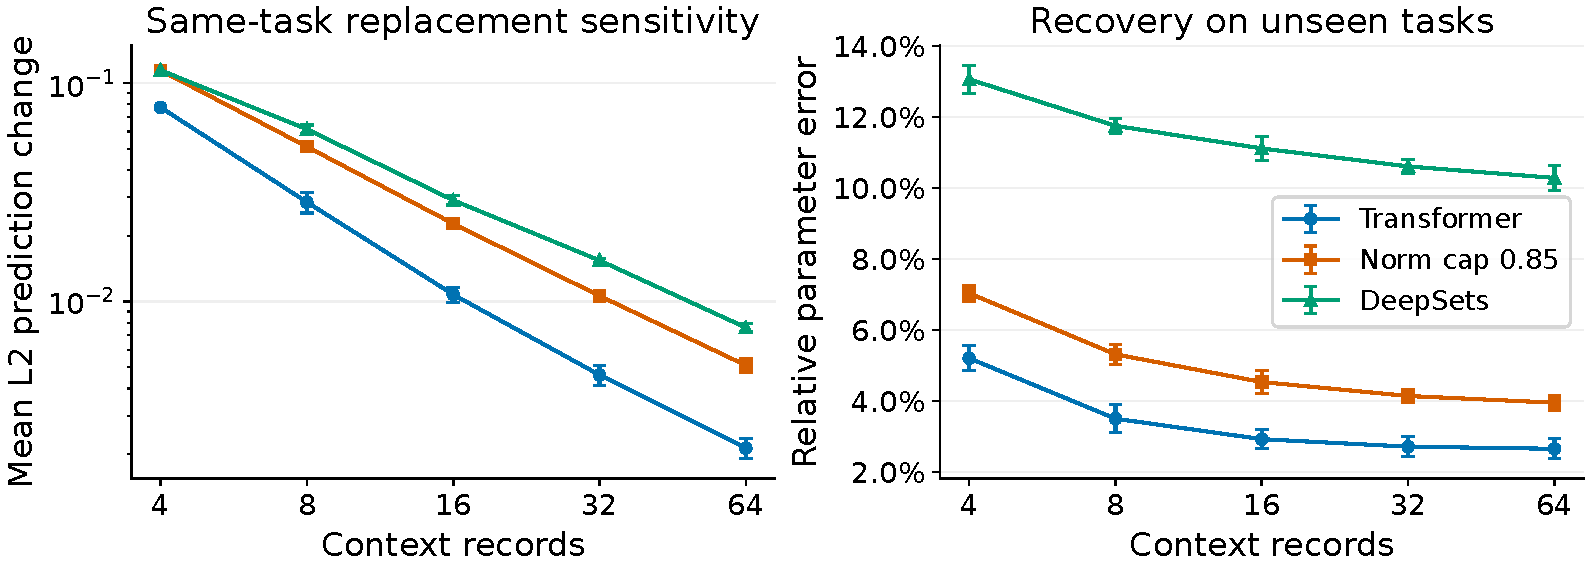
\includegraphics[width=.97\textwidth]{results/presentation/architecture.pdf}
\end{center}
\vspace{-1mm}
\small At \(m=64\), the original Transformer has
\(\Delta=0.00213\) and relative recovery error \(2.65\%\).
\vspace{1mm}

\small{\color{teal}The true task stays fixed, so a small response is compatible with accuracy.}
\source{Experiment D. Four valid same-task replacements per task and length.
The mean curves do not certify worst-case \(1/m\) scaling.}
\note{Target time 55 seconds, cumulative 12:10.
We first replace a record with another valid observation from
the same task. The correct parameter does not change.
The original Transformer's average sensitivity falls with context
length and its recovery error also improves. At length 64,
mean prediction change is about 0.00213 and relative recovery
error is 2.65 percent. It outperforms the other two learned
architectures under this schedule. This is consistent with
stability being useful for ordinary replacements. It does not
verify a worst-case asymptotic rate, because the plot averages
sampled changes. More importantly, these ordinary contexts
do not concentrate all identification in one record.
We next change the information structure.}
\end{frame}

% 14. 12:10--13:05
\begin{frame}{Nearly redundant contexts are harder to recover}
\begin{center}
\begin{tabular}{lccc}
\toprule
Context, \(m=16\)&Unique costs?&Minimum Gram eigenvalue&TF error\\
\midrule
Well-conditioned&Yes&\(0.03257\)&\(2.90\%\)\\[2mm]
Nearly redundant&Yes&\(3.72\times10^{-6}\)&\(13.65\%\)\\
\bottomrule
\end{tabular}
\end{center}
\vspace{5mm}
\begin{itemize}
\setlength{\itemsep}{3mm}
\item Both contexts mathematically determine the cost parameters.
\item Their mean demand is matched, but their observation spreads differ.
\item Nearly repeated equations supply weak information in one direction.
\end{itemize}
\vspace{3mm}
{\color{teal}Record count and unique identification do not ensure good learned recovery.}
\source{Experiment F. Seed means. The eigenvalue is the minimum across
generator-specific interior Gram matrices normalized by total context size.
Backup C gives all regimes.}
\note{Target time 55 seconds, cumulative 13:05.
Here both designs have sixteen observations and the same
task parameters. Each noiseless context uniquely determines
the costs, but one spreads its observations and the other
makes them nearly redundant. The small Gram eigenvalue
quantifies a weakly informed parameter direction.
The Transformer error increases from 2.90 to 13.65 percent.
Thus unique identification in exact arithmetic is insufficient
for good learned recovery. The designs match mean demand,
while their spreads necessarily differ. This does not by itself
isolate every feature-distribution effect. The next intervention
therefore holds the particular edited observation fixed.}
\end{frame}

% 15. 13:05--14:10
\begin{frame}{The same edit produces a larger response at high leverage}
\begin{columns}[c,onlytextwidth]
\column{.68\textwidth}
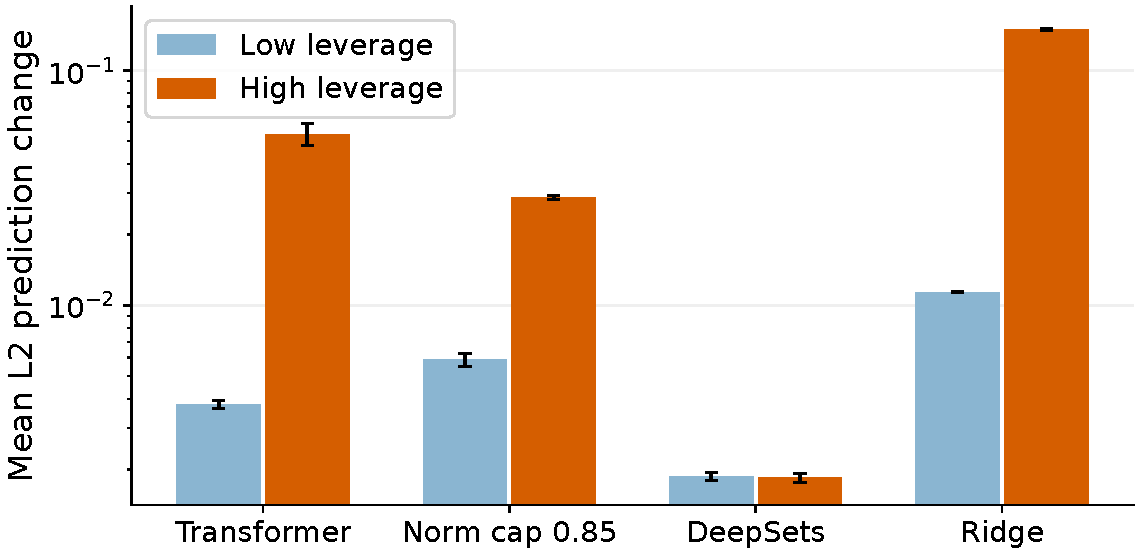
\includegraphics[width=\linewidth]{results/presentation/matched_response.pdf}
\column{.29\textwidth}
\small
Same focal record.

Same price displacement: \(0.02\).

Different backgrounds.
\vspace{4mm}

High / low response:
\[
\text{Transformer}:14.1\times
\]
\[
\text{Ridge}:13.1\times
\]
\end{columns}
\vspace{2mm}
\small{\color{teal}The surrounding information changes the model's response.}
\source{Experiment G. Price edit from \(\lambda-0.01\) to \(\lambda+0.01\).
The true task stays fixed. Mean focal hat leverage: 0.999 versus 0.133.}
\note{Target time 65 seconds, cumulative 14:10.
Leverage measures how much a record contributes to a regression
design relative to the rest. We keep the focal observation and
the price displacement fixed. The surrounding observations are
clustered or spread, making the focal record harder or easier to
replace informationally. The Transformer responds about fourteen
times more strongly in the high-leverage background. Ridge shows
a similar ratio, although its absolute response is larger.
DeepSets has almost no high-versus-low difference here.
These price perturbations leave the true task fixed and can be
viewed as measurement interventions. They establish output
responsiveness, not the correctness of a changed task estimate.
They also do not identify an internal attention mechanism.
We now return to the pair where the true parameter actually changes.}
\end{frame}

% 16. 14:10--15:25
\begin{frame}{On the identifying pair, the response remains incomplete}
\begin{columns}[c,onlytextwidth]
\column{.68\textwidth}
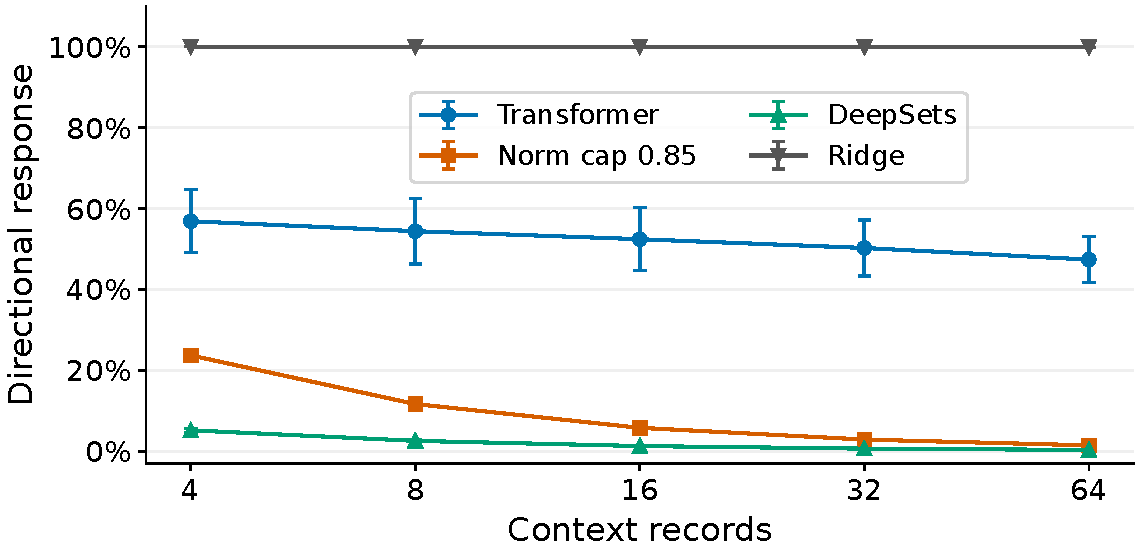
\includegraphics[width=\linewidth]{results/presentation/identifying_response.pdf}
\column{.29\textwidth}
\small
The valid pair from slide 11.

At \(m=64\):
\[
r_{\rm TF}=47.4\%
\]
\[
r_{\rm ridge}=99.9\%.
\]
Larger TF endpoint error:
\[
0.432.
\]
\end{columns}
\[
\small r=
\frac{\langle f(S')-f(S),\,\theta'-\theta\rangle}
{\norm{\theta'-\theta}^{2}}.
\]
\source{Experiment G. \(r=1\) means the correct response along the target
direction. Endpoint error is absolute Euclidean parameter error.}
\note{Target time 75 seconds, cumulative 15:25.
This is the exact economic-dispatch pair from slide eleven.
Both endpoints uniquely identify their different true parameters.
The reference at one hundred percent means the predicted
difference matches the true difference along the target direction.
It is not a prediction accuracy percentage, and it does not
by itself guarantee either endpoint is correct.
At length 64, Transformer directional response is 47.4 percent,
and its larger endpoint error averages 0.432. Ridge directional
response is 99.9 percent. Ridge demonstrates that these noiseless
contexts contain enough information to recover the task difference.
The Transformer responds substantially, but incompletely.
This is a finite-length measurement, not a consequence calculated
from our enormous C. To connect it quantitatively to theorem two,
we can instead use the response we actually measured.}
\end{frame}

% 17. 15:25--16:20
\begin{frame}{Theorem 2 also interprets the measured response}
% Derived from G identifying_pair_summary.csv; absolute parameter units.
\newcommand{\PairTargetGap}{1.265}
\newcommand{\PairMeanDelta}{0.603}
\newcommand{\PairErrorFloor}{0.331}
\newcommand{\PairObservedError}{0.432}

For each checkpoint, Theorem 2 gives
\[
\max(e_A,e_B)\ge\tfrac12(D-\Delta)_+.
\]
\begin{center}
\begin{tabular}{lr}
\toprule
Identifying pair at \(m=64\) & Parameter units\\
\midrule
True target separation \(D\)&\PairTargetGap\\
Measured mean response \(\overline\Delta\)&\PairMeanDelta\\
Implied lower bound on mean larger error&\(\ge\PairErrorFloor\)\\
Observed mean larger endpoint error&\PairObservedError\\
\bottomrule
\end{tabular}
\end{center}
\vspace{3mm}
{\color{teal}Measured response gives a finite-length error constraint without using \(C\).}
\source{Computed from saved G summaries, three original Transformer checkpoints.
Averaging gives \(\overline{\max(e_A,e_B)}\ge(D-\overline\Delta)_+/2\).
This is a geometric consistency check.}
\note{Target time 55 seconds, cumulative 16:20.
Theorem two can use an observed response, rather than the loose
architectural certificate. The true target separation is about
1.265. Mean prediction change across the three checkpoints is
about 0.603. The resulting lower bound on the mean larger
endpoint error is about 0.331. The observed value is 0.432.
These quantities use absolute parameter units, not relative
error or the directional-response percentage from the previous slide.
The inequality holds checkpoint by checkpoint and survives averaging.
This is a useful way to interpret the under-response. It is a
geometric requirement, not evidence that the worst-case C caused
the trained model's behavior.}
\end{frame}

\section{Conclusion}
% 18. 16:20--17:25
\begin{frame}{Contribution and scope}
\begin{columns}[T,onlytextwidth]
\column{.48\textwidth}
{\large What this project establishes}
\begin{itemize}
\setlength{\itemsep}{3mm}
\item Architecture-specific stability verification.
\item Valid, individually identifying dispatch pairs.
\item Controlled response and recovery measurements.
\end{itemize}
\column{.48\textwidth}
{\large What limits the conclusion}
\begin{itemize}
\setlength{\itemsep}{3mm}
\item Loose constants and repeated-record worst cases.
\item Three seeds and two synthetic generators.
\item Behavioral evidence leaves internal mechanisms unresolved.
\end{itemize}
\end{columns}
\vspace{5mm}
\small Li et al. analyze query prediction and stability-based generalization.
We examine recovery when identifying information is concentrated.
\source{Li et al. (2023), Theorem 3.2 and Appendix B.
Theorem 2 is a generic triangle-inequality argument.
Fixed-compute task-count benefits remain inconclusive (Backup D).}
\note{Target time 65 seconds, cumulative 17:25.
The theoretical novelty should be described carefully.
Li and colleagues already establish a Transformer stability
argument and connect stability to generalization. We adapt the
reasoning to our implemented mean-pooled encoder with residual
and normalization maps. The recovery lower bound itself is a
basic triangle-inequality consequence. Our concrete contribution
connects that architectural verification to valid identifying
dispatch pairs and controlled measurements of information,
response and recovery. The worst-case family deliberately repeats
records. The norm constant is loose, and finite experiments use
only three seeds and two generators. We also do not establish a
task-count benefit at fixed compute. Those controls are in backup.
These qualifications define the claim we can defend.}
\end{frame}

% 19. 17:25--18:00
\begin{frame}{Accurate recovery requires sufficient response}
\begin{enumerate}
\setlength{\itemsep}{5mm}
\item A long context can leave one record responsible for a whole parameter direction.
\item Theorem 1 bounds possible response.
Theorem 2 bounds the response required for recovery.
\item The trained Transformer responds to context information,
but its identifying response can remain insufficient.
\end{enumerate}
\vspace{6mm}
{\color{teal}\large Sensitivity is meaningful when we ask which information changed
and whether the resulting estimate is accurate.}
\note{Target time 35 seconds, cumulative 18:00.
Return to the line example. Many repeated records do not replace
the one observation that determines the slope. The two theorems
compare an architectural response ceiling with the response
required to recover different truths. The experiments show
information-dependent responsiveness, together with incomplete
recovery on the identifying pair. The question is therefore
whether the model responds enough to the information needed
for the task.}
\end{frame}

\appendix
\setbeamertemplate{footline}{\hspace{8mm}\textcolor{muted}{\scriptsize Backup}\hfill
\textcolor{muted}{\scriptsize Fei Zhang\quad CS 886}\hspace{8mm}\vspace{3mm}}

\begin{frame}[noframenumbering]{Backup A. The attention Jacobian step}
\small
Fixed affine query and key maps give
\[
|s_{ij}-s_{ij}'|\le c_q e_i+c_k e_j.
\]
Along the score segment every probability is at most \(e^{2B}/m\).
For \(J(p)=\operatorname{diag}(p)-pp^\top\),
\[
\sum_k|J_{kj}|=2p_j(1-p_j)\le2p_j.
\]
Integration therefore gives
\[
\|p_i-p_i'\|_1\le2e^{2B}(c_qe_i+c_k\bar e).
\]
Changing weights with values fixed costs at most \(V_0\|p_i-p_i'\|_1\).
Changing values with weights fixed costs at most \(ve^{2B}\bar e\).
Averaging rows gives \(L_{\rm att}\bar e\).
\source{Finite constants depend on weight and hidden-state bounds.
The report appendix includes multihead concatenation and the output projection.}
\end{frame}
\begin{frame}[noframenumbering]{Backup B. LayerNorm derivative bound}
\small
Let \(P\) center a width-\(p\) row and set
\[
g(z)=\frac{z}{(\|z\|_2^2/p+\eta)^{1/2}},\qquad \eta>0.
\]
The derivative eigenvalues are
\[
\lambda_{\rm tangential}
 =(\|z\|_2^2/p+\eta)^{-1/2},
\qquad
\lambda_{\rm radial}
 =\eta(\|z\|_2^2/p+\eta)^{-3/2}.
\]
Both are at most \(1/\sqrt{\eta}\), and \(\|P\|=1\).
\[
\mathrm{LN}(h)=\operatorname{diag}(\gamma)\,g(Ph)+\beta
\quad\Longrightarrow\quad
L_{\rm LN}\le\frac{\|\gamma\|_\infty}{\sqrt{\eta}}.
\]
\source{Applies to the implemented post-residual LayerNorm with \(\eta=10^{-5}\).}
\end{frame}

\begin{frame}[noframenumbering]{Backup C. All context-information regimes}
\begin{center}
\begin{tabular}{lrrr}
\toprule
Context at \(m=16\)&Minimum Gram eigenvalue&Set diameter&TF error\\
\midrule
Well-conditioned&\(0.03257\)&0&2.90\%\\
Nearly redundant&\(3.72\times10^{-6}\)&0&13.65\%\\
Mixed&\(0.02429\)&0&3.72\%\\
Boundary-heavy&0&1.056&17.64\%\\
\bottomrule
\end{tabular}
\end{center}
\vspace{4mm}
\[
H_i=\frac1m\sum_{t:\,s_{it}=\mathrm{int}}u_{it}u_{it}^{\top},
\qquad u_{it}=(1,x_{it})^\top.
\]
\small The eigenvalue is \(\min_i\lambda_{\min}(H_i)\).
Interior contexts share mean demand; their output spreads differ.
\source{Experiment F. Diameter refers to the boxed KKT-admissible parameter set. Values are seed means.}
\end{frame}

\begin{frame}[noframenumbering]{Backup D. Task-count and training-budget controls}
\begin{center}
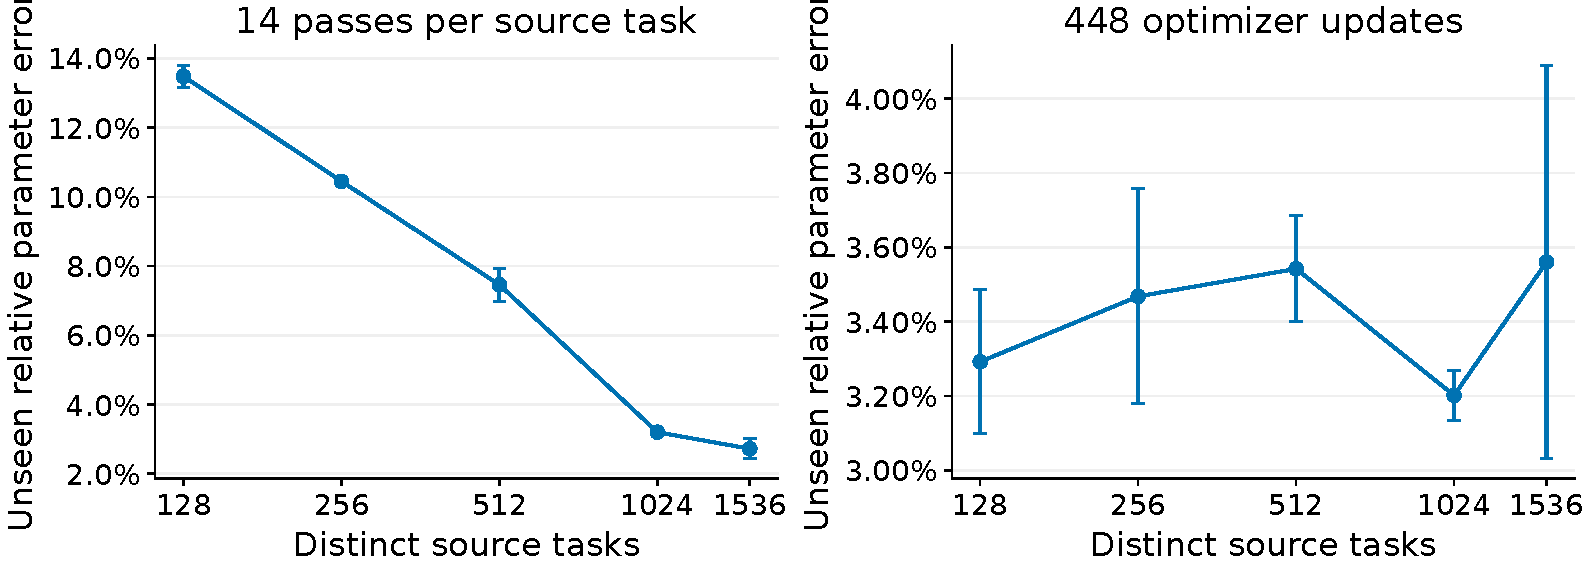
\includegraphics[width=.97\textwidth]{results/presentation/transfer.pdf}
\end{center}
\small The equal-pass sweep spends 56--672 updates as source-task count grows.

\source{Experiment E, evaluation context length 32. Under 448 updates, target error is nonmonotonic across task counts.}
\end{frame}

\begin{frame}[noframenumbering]{Backup E. Information spread across multiple records}
\begin{center}
\begin{tabular}{rrrr}
\toprule
Identifying records \(k\)&TF direction recovered&Largest path step&Larger TF error\\
\midrule
1&50.0\%&0.301&0.281\\
2&52.3\%&0.206&0.272\\
4&53.8\%&0.128&0.266\\
8&54.7\%&0.074&0.262\\
\bottomrule
\end{tabular}
\end{center}
\vspace{4mm}
\small 192 valid task pairs, \(m=64\), target separation 0.6 and focal
price difference 0.09.

\vspace{3mm}
Telescoping a bounded-input path gives
\[
\norm{f(S')-f(S)}\le\frac{kC}{m}.
\]
\source{Completed follow-up. Intermediate price mixtures on the path can be inconsistent with a single noiseless task.}
\end{frame}

\begin{frame}[noframenumbering]{Backup F. Independent noise on every context price}
\begin{center}
\begin{tabular}{lrr}
\toprule
Context at noise SD \(0.04\)&Transformer error&Ridge error\\
\midrule
Well-conditioned&3.87\%&2.39\%\\
Nearly redundant&13.67\%&15.28\%\\
Boundary-heavy&17.41\%&15.50\%\\
\bottomrule
\end{tabular}
\end{center}
\vspace{5mm}
\begin{itemize}
\item Gaussian noise changes prices while dispatch and status stay exact.
\item Ridge uses noisy validation tasks and clipping to the cost box.
\item The frozen Transformer was trained on clean contexts.
\end{itemize}
\source{Completed follow-up. Three seeds, four noise draws per task, length 16.}
\end{frame}

\begin{frame}[noframenumbering]{Backup G. Supporting task-level transfer bound}
\small
For IID source tasks and a fixed hypothesis class, define
\[
L_\theta(f)=\mathbb E_{S\sim P_\theta^m}
  \left[\frac14\sum_{j=1}^{4}
    \left(\frac{f_j(S)-\theta_j}{\mathrm{span}_j}\right)^2\right].
\]
With an \(\varepsilon\)-cover of the task-risk functions in sup norm of
size \(N_\varepsilon\), with probability at least \(1-\delta\),
\[
\left|\mathbb E_\theta L_\theta(f)-\frac1T\sum_{t=1}^{T}L_{\theta_t}(f)\right|
\le2\varepsilon+
\sqrt{\frac{\log(2N_\varepsilon/\delta)}{2T}}.
\]
Hoeffding at each center, a union bound, and two approximation terms prove the claim.
\source{Standard uniform convergence argument. The class and same-distribution assumptions determine its scope.}
\end{frame}

\begin{frame}[noframenumbering]{Backup H. References and reproducibility}
\footnotesize
\begin{itemize}
\setlength{\itemsep}{3mm}
\item Li, Ildiz, Papailiopoulos and Oymak (2023).
\emph{Transformers as Algorithms}. ICML.
\href{https://proceedings.mlr.press/v202/li23l.html}{Paper}
\item Keshavarz, Wang and Boyd (2011).
\emph{Imputing a Convex Objective Function}. IEEE MSC.
\item Aky\"urek et al.\ (2023).
\emph{What Learning Algorithm Is In-Context Learning?} ICLR.
\item Chakraborty, Luo and Barber (2026).
\emph{Stability and Accuracy Trade-offs in Statistical Estimation}.
\end{itemize}
\vspace{4mm}
\href{https://github.com/feizhanguwaterloo/Stability-and-Information-Sensitivity-in-Transformer-In-Context-Inverse-Learning}
{\textcolor{teal}{Project repository with code, tests, configurations, results and report source}}
\end{frame}
\end{document}
